In this appendix I examine the effect of the choices of
hyperparameters on the results of two of the experiments discussed in
the body of the dissertation: the synthetic cocktail party experiment
in Chapter \ref{chapter:cocktail-party}, and the Bach chorale
experiment in Chapter \ref{chapter:music}.


\section{Synthetic Cocktail Party Data}
The results reported in Chapter \ref{chapter:cocktail-party} are based
on the binary state, linear-Gaussian form of the HDP-HMM-LT, with a
Laplace similarity kernel defined over Hamming distances between
binary state vectors.  All hyperparameters of the HDP, as well as the
scale parameter of the similarity kernel, are sampled during
inference; however, the hyperpriors on the two HDP concentration
parameters, $\alpha$ and $\gamma$, and on the variance, $\sigma^2$ of
the Gaussian noise, need to be set by hand.  In this section I explore
the effect of different choices of hyperparameters for these priors.

The HDP-HMM and the HDP-HMM-LT as used in their binary state, linear-Gaussian forms, are defined with the following generative model:
\begin{align*}
  \beta &\sim \GEM{\gamma} \\
  \pi_{jj'} &\stackrel{i.i.d}{\sim} \Gamm{\alpha\beta_{j'}}{\phi_{jj'}^{-1}} \quad j' = 1, 2, \dots \\
  z_{t} \given z_{t-1} &\sim \Disc{\pi_{z_t,\cdot}} \\
  y_{tk} \given z_t, \theta, w_k &\stackrel{ind.}{\sim} \Norm{w_k^{\sf T} \theta_{z_t}}{h_k^{-1}}
\end{align*}
where in the non-LT HDP-HMM case all $\phi_{jj'}$ are identically 1, while in the LT case, we have
\begin{align*}
  \phi_{jj'} := \exp(-\lambda \Delta_{j,j'})
\end{align*}
where $\Delta_{jj'} = \sum_{d} \abs{\theta_{jd} - \theta_{jd'}}$ 
is the Hamming distance between $\theta_j$ and $\theta_{j'}$.

In the case of the Binary Factorial HMM, the binary transition
matrices for each were also constructed using independent HDP priors
with concentration parameters $\gamma$ and $\alpha$.

We have the following top-level priors:
\begin{align*}
  \gamma &\sim \Gamm{a_{\gamma}}{b_{\gamma}} \\
  \alpha &\sim \Gamm{a_{\alpha}}{b_{\alpha}} \\
  h &\sim \Gamm{a_{h}}{b_{h}} \\
  \lambda &\sim \Exp{b_{\lambda}}
\end{align*}
where all distributions are parameterized in terms of shape $a$ and rate $b$.

The reference value for all shape and rate parameters is 0.1.  The
parametric variants explored in the results reported here are listed
in Table \ref{tab:cocktail-param-values}.

\begin{table}
  \centering
  \begin{tabular}{|r|c|c|c|c|c|c|c|} \hline
    Expt. & $a_\gamma$ & $b_{\gamma}$ & $a_\alpha$ & $b_{\alpha}$ & $a_h$ &
    $b_h$ & $b_\lambda$ \\ \hline
    1 & {\bf 0.01} & {\bf 0.01} & 0.1 & 0.1 & 0.1 & 0.1 & 0.1 \\
    2 & {\bf 0.01} & {\bf 5.0} & 0.1 & 0.1 & 0.1 & 0.1 & 0.1 \\
    3 & {\bf 5.0} & {\bf 0.01} & 0.1 & 0.1 & 0.1 & 0.1 & 0.1 \\
    4 & {\bf 5.0} & {\bf 5.0} & 0.1 & 0.1 & 0.1 & 0.1 & 0.1 \\
    5 & 0.1 & 0.1 & {\bf 0.01} & {\bf 0.01} & 0.1 & 0.1 & 0.1 \\
    6 & 0.1 & 0.1 & {\bf 0.01} & {\bf 5.0} & 0.1 & 0.1 & 0.1 \\
    7 & 0.1 & 0.1 & {\bf 5.0} & {\bf 0.01} & 0.1 & 0.1 & 0.1 \\
    8 & 0.1 & 0.1 & {\bf 5.0} & {\bf 5.0} & 0.1 & 0.1 & 0.1 \\
    9 & 0.1 & 0.1 & 0.1 & 0.1 & {\bf 0.01} & {\bf 0.01} & 0.1 \\
    10 & 0.1 & 0.1 & 0.1 & 0.1 & {\bf 0.01} & {\bf 5.0} & 0.1 \\
    11 & 0.1 & 0.1 & 0.1 & 0.1 & {\bf 5.0} & {\bf 0.01} & 0.1 \\
    12 & 0.1 & 0.1 & 0.1 & 0.1 & {\bf 5.0} & {\bf 5.0} & 0.1 \\ \hline
  \end{tabular}
  \caption{Hyperprior parameter values explored in the synthetic
    cocktail party setting}
  \label{tab:cocktail-param-values}
\end{table}

For the most part the hyperparameters make little difference to the
pattern of results, with the exception that when the $b_\alpha$ or
$b_{\gamma}$ parameters are too high, and hence the prior is holding
$\alpha$ and $\gamma$ down at smaller values.  The prior mean of a
Gamma distribution is $a/b$
and the prior variance is $a/b^2$, so when $a$ is 0.01 and $b$ is 5,
the mean is $0.002$ and the standard deviation is $0.02$, which means
that even 1.0 is nearly 50 standard deviations above the mean; when $a
= b = 5.0$, the mean is 1 and the standard deviation is less than
0.5.  Under these conditions, all of the HDP models suffer: in the
case of $\gamma$ being too small, they
concentrate their mass too tightly in a few states overall, and in the
case of $\alpha$ being too small, the transition matrices become too
close to deterministic (with too few states in each row having
non-negligible probability mass).  
However, under all less restrictive priors, the pattern of results
reported in Chapter \ref{chapter:cocktail-party} holds.

\begin{figure}[tb]
  \centering
  \begin{minipage}{0.75\textwidth}
  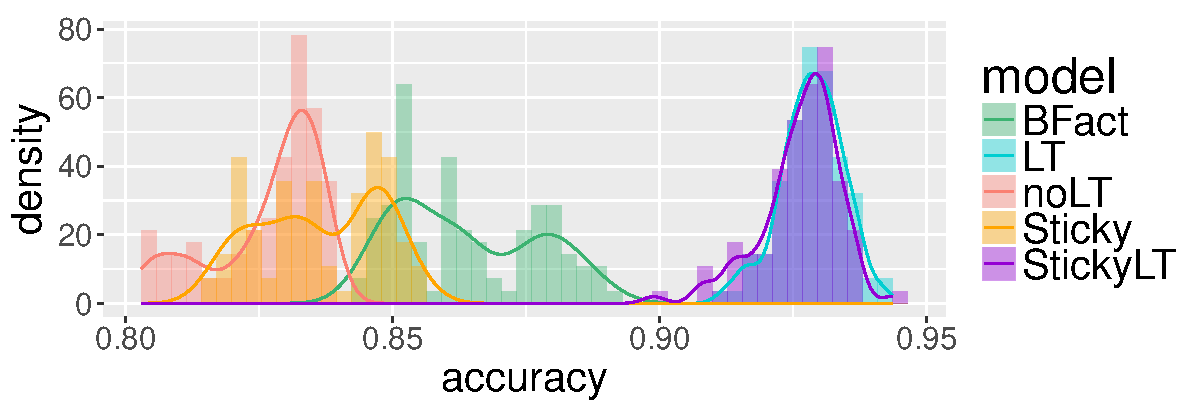
\includegraphics[width = \textwidth]{fig/cocktail/synth_s16_m12/hyper_gamma/h10.0_nocs_cp0/a0p01b0p01/accuracy_density.pdf}
\end{minipage}

\begin{minipage}{0.75\textwidth}
  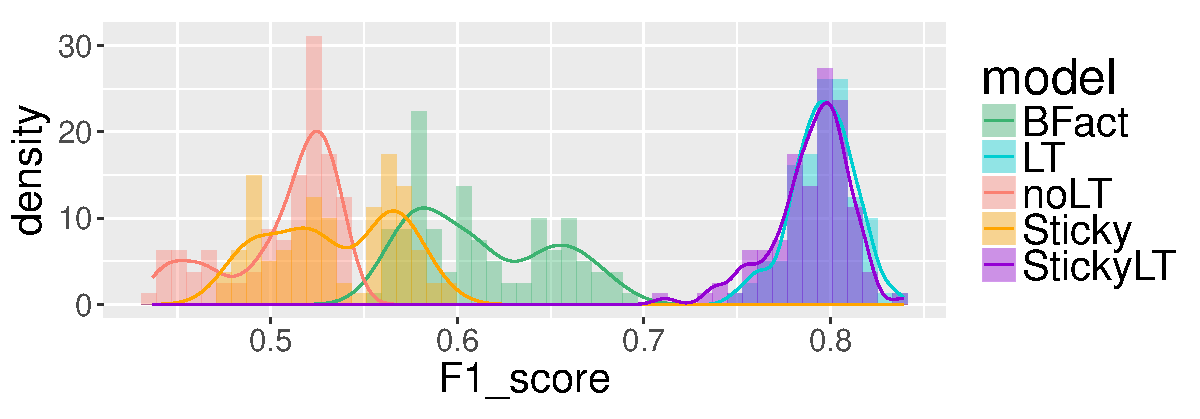
\includegraphics[width = \textwidth]{fig/cocktail/synth_s16_m12/hyper_gamma/h10.0_nocs_cp0/a0p01b0p01/F1_score_density.pdf}
\end{minipage}

\begin{minipage}{0.75\textwidth}
  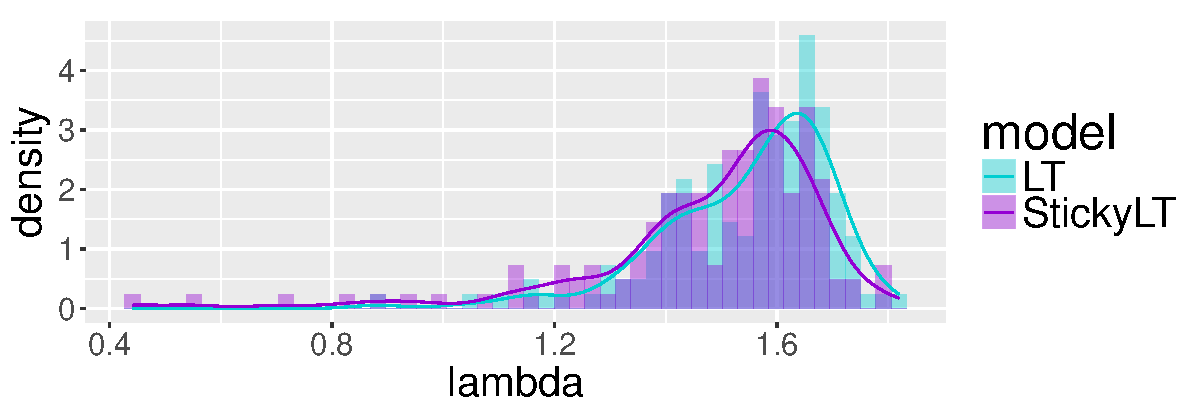
\includegraphics[width = \textwidth]{fig/cocktail/synth_s16_m12/hyper_gamma/h10.0_nocs_cp0/a0p01b0p01/lambda_density.pdf}
\end{minipage}

\begin{minipage}{0.75\textwidth}
  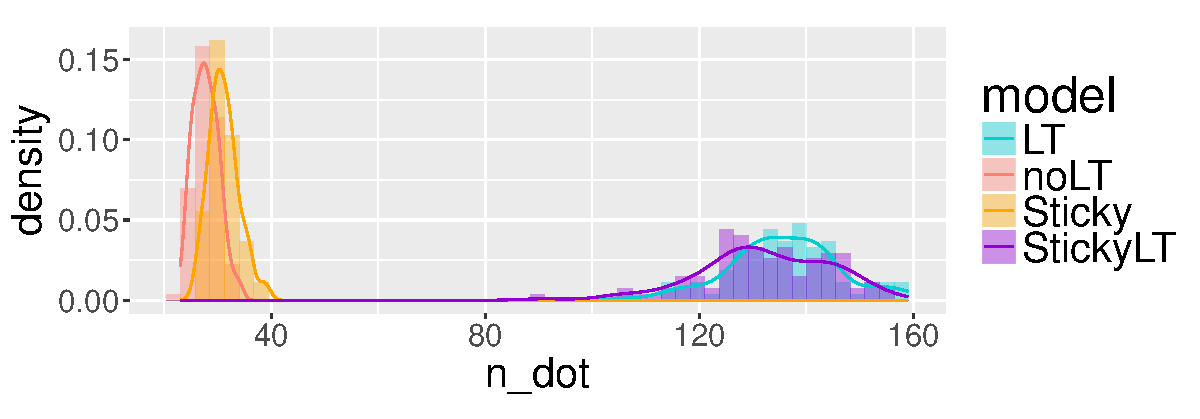
\includegraphics[width = \textwidth]{fig/cocktail/synth_s16_m12/hyper_gamma/h10.0_nocs_cp0/a0p01b0p01/n_dot_density.pdf}
\end{minipage}
\caption{Metrics for run 1: $\gamma \sim \Gamm{0.01}{0.01}$}
\end{figure}

\begin{figure}[tb]
% \vskip 0.1in
\begin{center}
  \centerline{\includegraphics[width = \textwidth, height = 0.2\textwidth]{fig/cocktail/synth_s16_m12/hyper_gamma/h10.0_nocs_cp0/a0p01b0p01/groundtruth.pdf}}
  \centerline{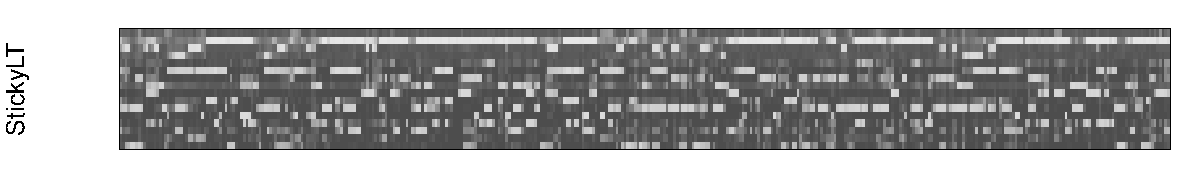
\includegraphics[width = \textwidth, height = 0.2\textwidth]{fig/cocktail/synth_s16_m12/hyper_gamma/h10.0_nocs_cp0/a0p01b0p01/StickyLT_hdp_hmm_w0_agamma0p01_bgamma0p01/binary_state.pdf}}
  \centerline{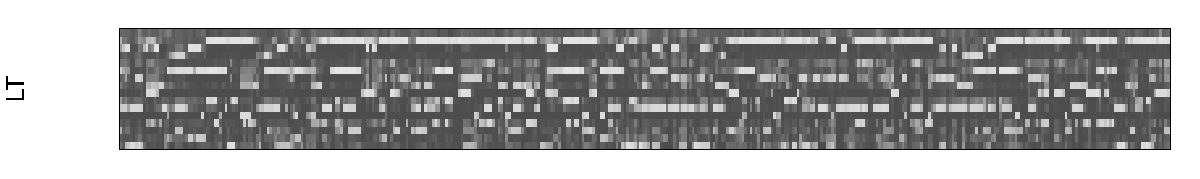
\includegraphics[width = \textwidth, height = 0.2\textwidth]{fig/cocktail/synth_s16_m12/hyper_gamma/h10.0_nocs_cp0/a0p01b0p01/LT_hdp_hmm_w0_agamma0p01_bgamma0p01/binary_state.pdf}}
  \centerline{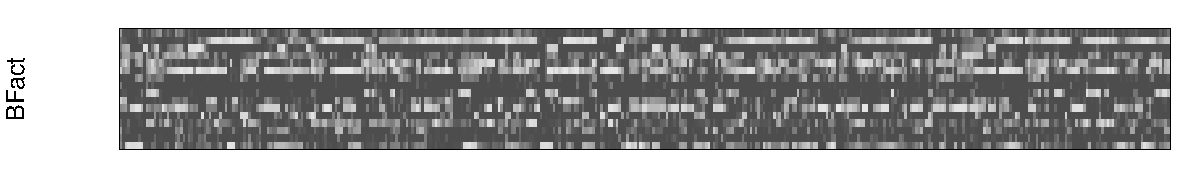
\includegraphics[width = \textwidth, height = 0.2\textwidth]{fig/cocktail/synth_s16_m12/hyper_gamma/h10.0_nocs_cp0/a0p01b0p01/BFact_hmm_w0_agamma0p01_bgamma0p01/binary_state.pdf}}
  \centerline{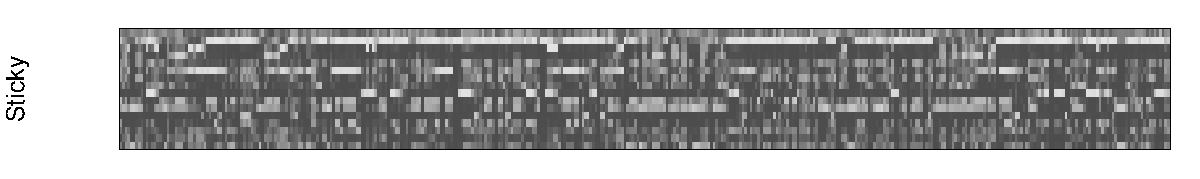
\includegraphics[width = \textwidth, height = 0.2\textwidth]{fig/cocktail/synth_s16_m12/hyper_gamma/h10.0_nocs_cp0/a0p01b0p01/Sticky_hdp_hmm_w0_agamma0p01_bgamma0p01/binary_state.pdf}}
  \centerline{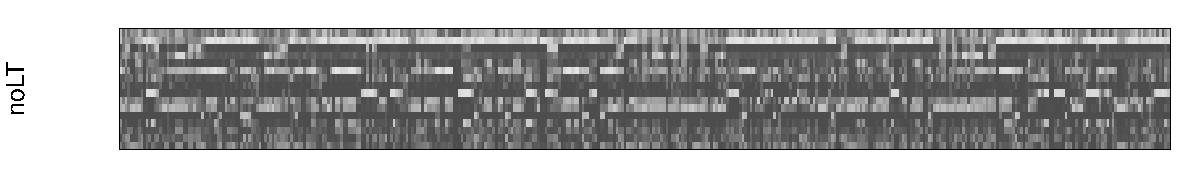
\includegraphics[width = \textwidth, height = 0.2\textwidth]{fig/cocktail/synth_s16_m12/hyper_gamma/h10.0_nocs_cp0/a0p01b0p01/noLT_hdp_hmm_w0_agamma0p01_bgamma0p01/binary_state.pdf}}
\caption{Binary speaker matrices for run 1: $\gamma \sim \Gamm{0.01}{0.01}$}
\end{center}
\end{figure}


\begin{figure}[tb]
  \centering
  \begin{minipage}{0.75\textwidth}
  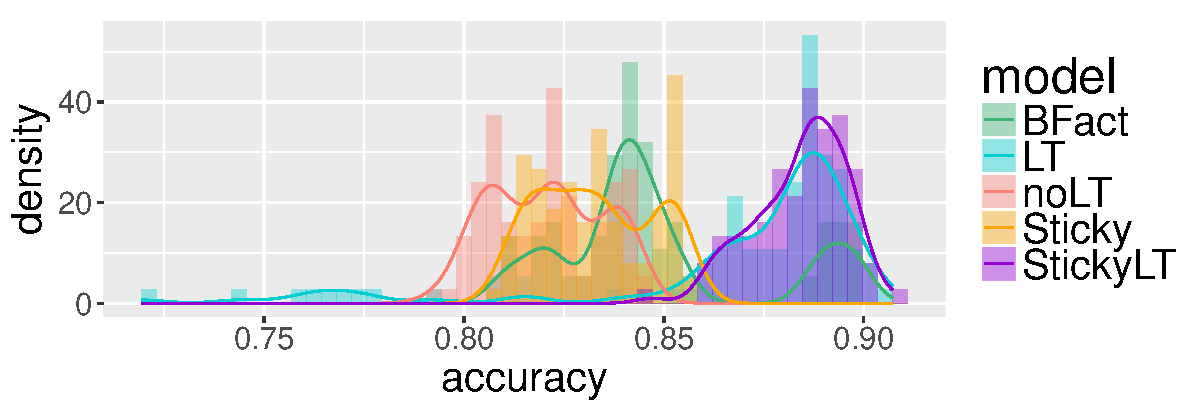
\includegraphics[width = \textwidth]{fig/cocktail/synth_s16_m12/hyper_gamma/h10.0_nocs_cp0/a0p01b5/accuracy_density.pdf}
\end{minipage}

\begin{minipage}{0.75\textwidth}
  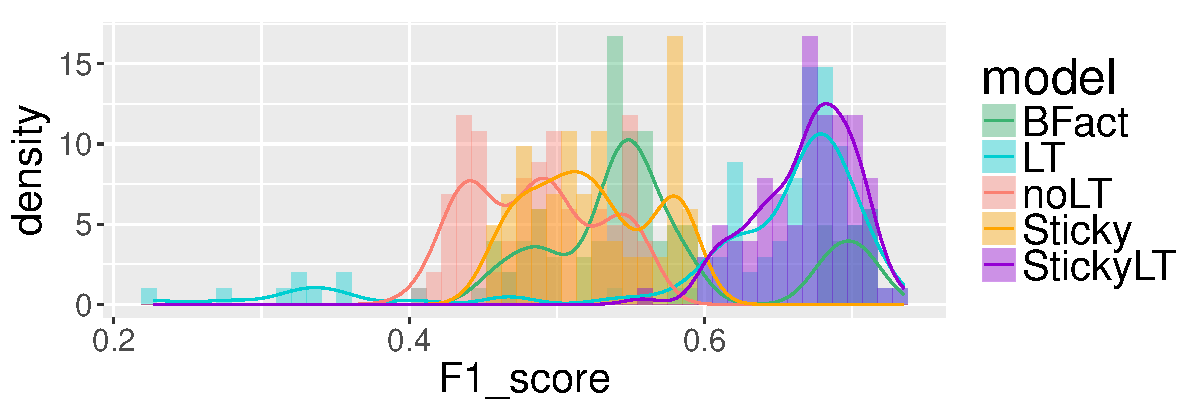
\includegraphics[width = \textwidth]{fig/cocktail/synth_s16_m12/hyper_gamma/h10.0_nocs_cp0/a0p01b5/F1_score_density.pdf}
\end{minipage}

\begin{minipage}{0.75\textwidth}
  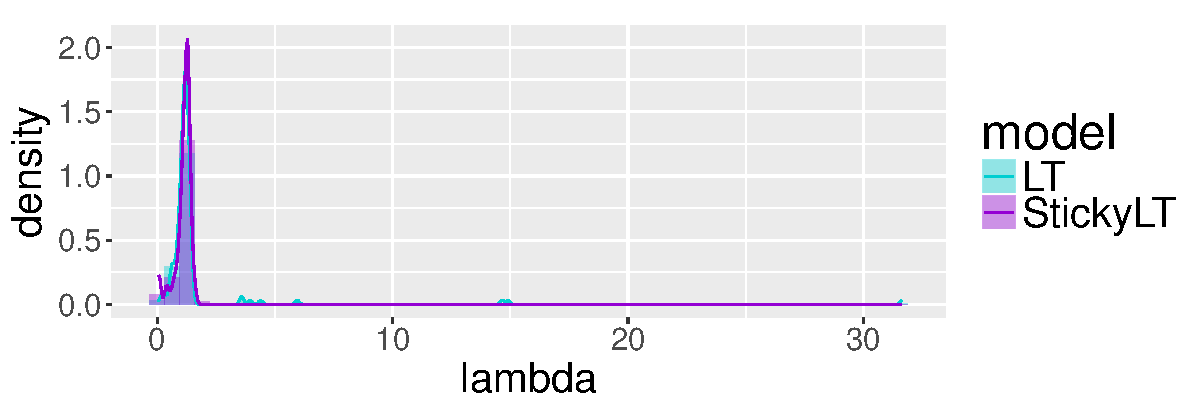
\includegraphics[width = \textwidth]{fig/cocktail/synth_s16_m12/hyper_gamma/h10.0_nocs_cp0/a0p01b5/lambda_density.pdf}
\end{minipage}

\begin{minipage}{0.75\textwidth}
  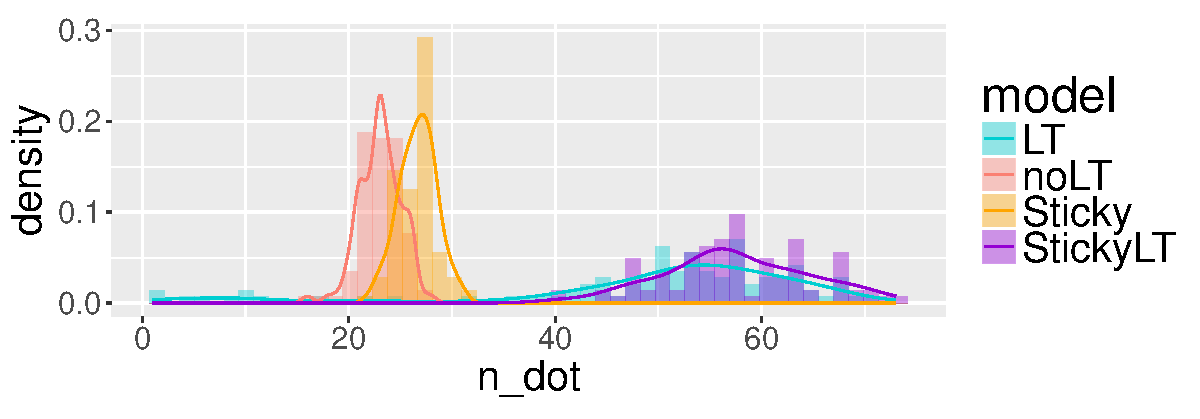
\includegraphics[width = \textwidth]{fig/cocktail/synth_s16_m12/hyper_gamma/h10.0_nocs_cp0/a0p01b5/n_dot_density.pdf}
\end{minipage}
\caption{Metrics for run 2: $\gamma \sim \Gamm{0.01}{5}$}
\end{figure}

\begin{figure}[tb]
% \vskip 0.1in
\begin{center}
  \centerline{\includegraphics[width = \textwidth, height = 0.2\textwidth]{fig/cocktail/synth_s16_m12/hyper_gamma/h10.0_nocs_cp0/a0p01b5/groundtruth.pdf}}
  \centerline{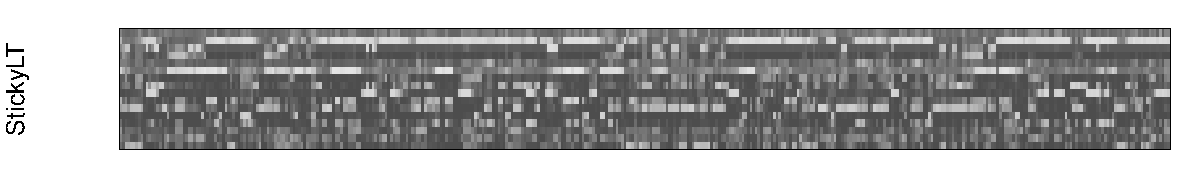
\includegraphics[width = \textwidth, height = 0.2\textwidth]{fig/cocktail/synth_s16_m12/hyper_gamma/h10.0_nocs_cp0/a0p01b5/StickyLT_hdp_hmm_w0_agamma0p01_bgamma5/binary_state.pdf}}
  \centerline{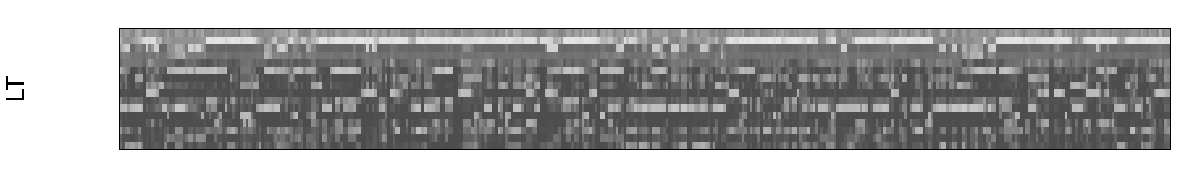
\includegraphics[width = \textwidth, height = 0.2\textwidth]{fig/cocktail/synth_s16_m12/hyper_gamma/h10.0_nocs_cp0/a0p01b5/LT_hdp_hmm_w0_agamma0p01_bgamma5/binary_state.pdf}}
  \centerline{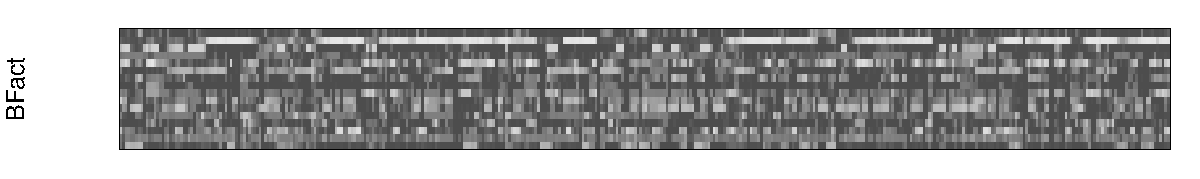
\includegraphics[width = \textwidth, height = 0.2\textwidth]{fig/cocktail/synth_s16_m12/hyper_gamma/h10.0_nocs_cp0/a0p01b5/BFact_hmm_w0_agamma0p01_bgamma5/binary_state.pdf}}
  \centerline{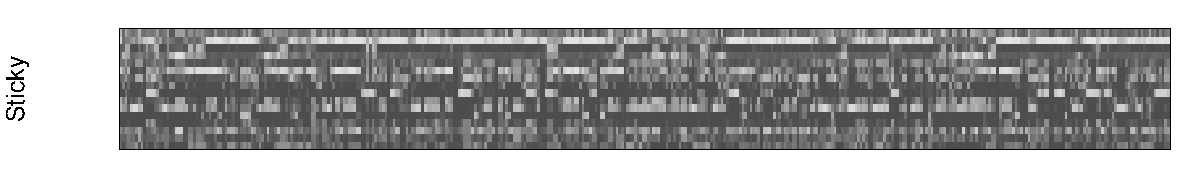
\includegraphics[width = \textwidth, height = 0.2\textwidth]{fig/cocktail/synth_s16_m12/hyper_gamma/h10.0_nocs_cp0/a0p01b5/Sticky_hdp_hmm_w0_agamma0p01_bgamma5/binary_state.pdf}}
  \centerline{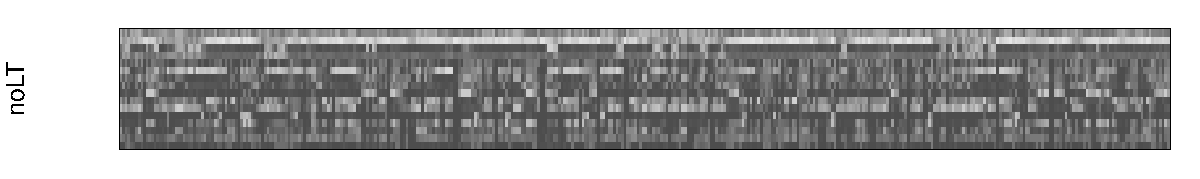
\includegraphics[width = \textwidth, height = 0.2\textwidth]{fig/cocktail/synth_s16_m12/hyper_gamma/h10.0_nocs_cp0/a0p01b5/noLT_hdp_hmm_w0_agamma0p01_bgamma5/binary_state.pdf}}
\caption{Binary speaker matrices for run 2: $\gamma \sim \Gamm{0.01}{5}$}
\end{center}
\end{figure}

\begin{figure}[tb]
  \centering
  \begin{minipage}{0.75\textwidth}
  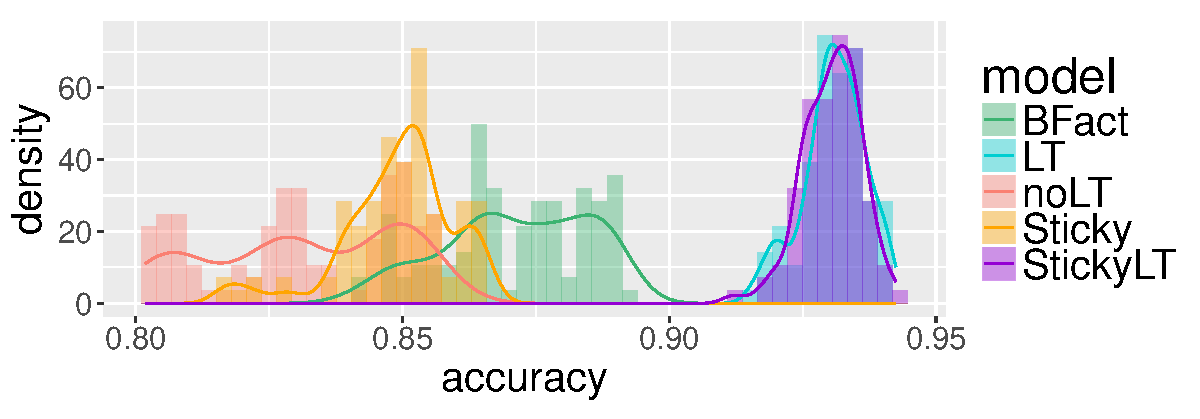
\includegraphics[width = \textwidth]{fig/cocktail/synth_s16_m12/hyper_gamma/h10.0_nocs_cp0/a5b0p01/accuracy_density.pdf}
\end{minipage}

\begin{minipage}{0.75\textwidth}
  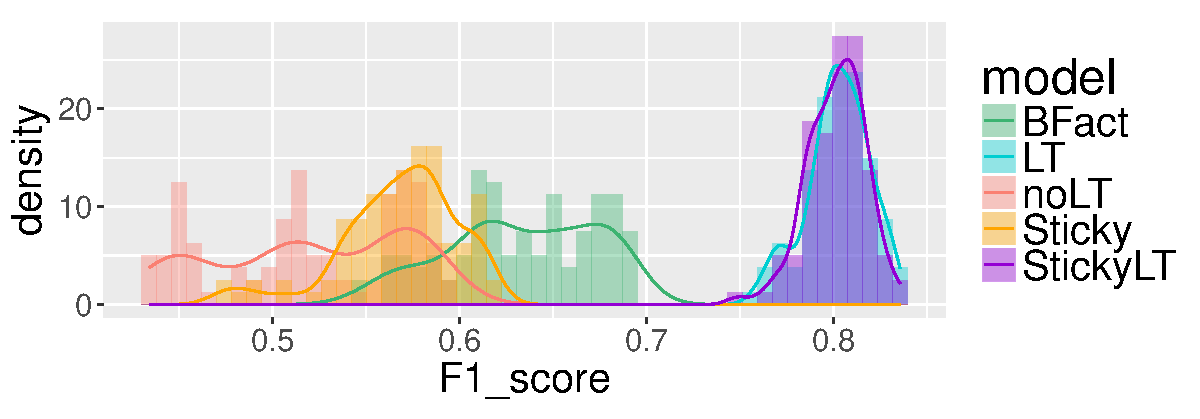
\includegraphics[width = \textwidth]{fig/cocktail/synth_s16_m12/hyper_gamma/h10.0_nocs_cp0/a5b0p01/F1_score_density.pdf}
\end{minipage}

\begin{minipage}{0.75\textwidth}
  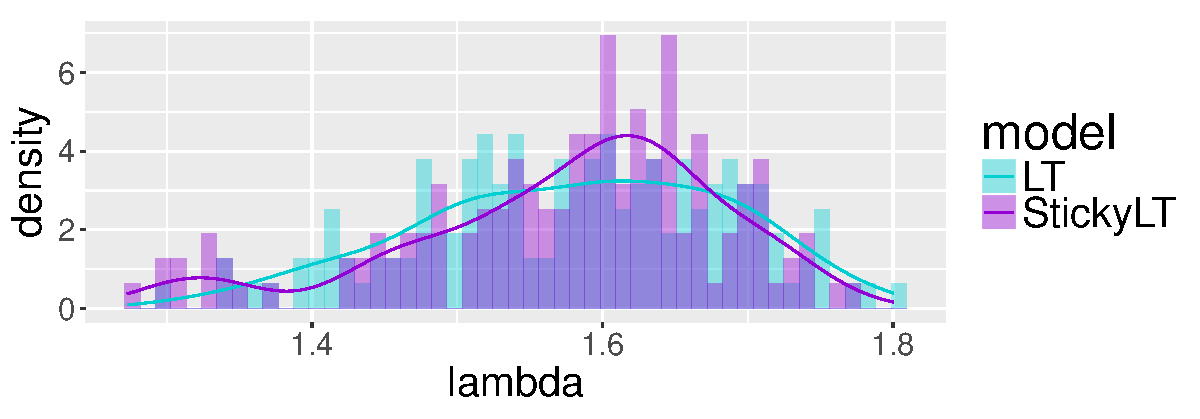
\includegraphics[width = \textwidth]{fig/cocktail/synth_s16_m12/hyper_gamma/h10.0_nocs_cp0/a5b0p01/lambda_density.pdf}
\end{minipage}

\begin{minipage}{0.75\textwidth}
  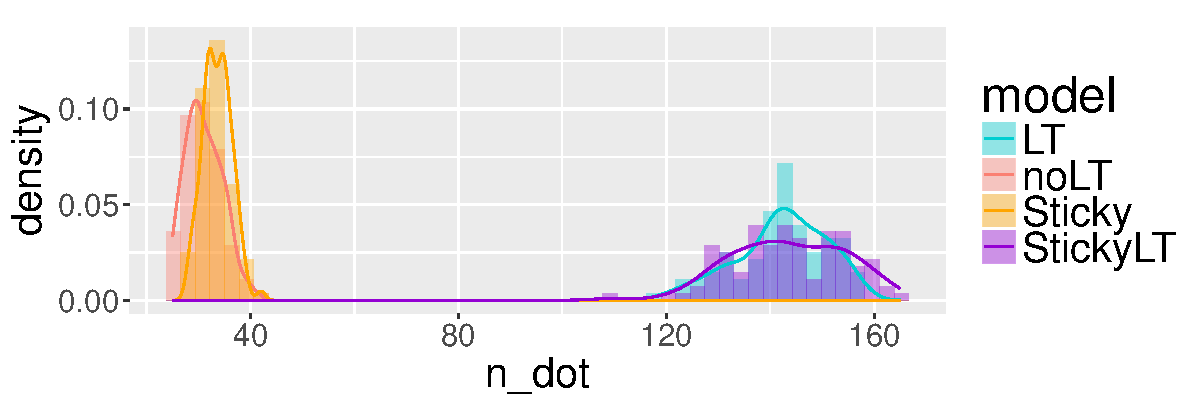
\includegraphics[width = \textwidth]{fig/cocktail/synth_s16_m12/hyper_gamma/h10.0_nocs_cp0/a5b0p01/n_dot_density.pdf}
\end{minipage}
\caption{Metrics for run 3: $\gamma \sim \Gamm{5}{0.01}$}
\end{figure}

\begin{figure}[tb]
% \vskip 0.1in
\begin{center}
  \centerline{\includegraphics[width = \textwidth, height = 0.2\textwidth]{fig/cocktail/synth_s16_m12/hyper_gamma/h10.0_nocs_cp0/a5b0p01/groundtruth.pdf}}
  \centerline{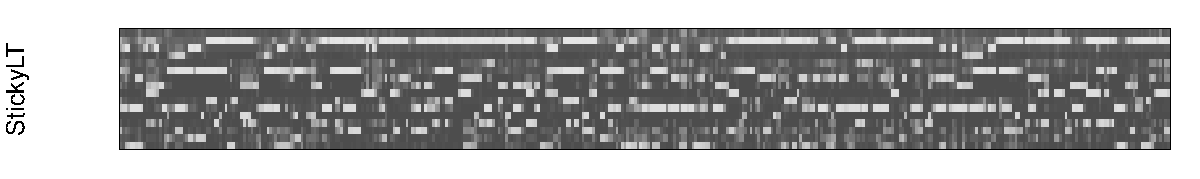
\includegraphics[width = \textwidth, height = 0.2\textwidth]{fig/cocktail/synth_s16_m12/hyper_gamma/h10.0_nocs_cp0/a5b0p01/StickyLT_hdp_hmm_w0_agamma5_bgamma0p01/binary_state.pdf}}
  \centerline{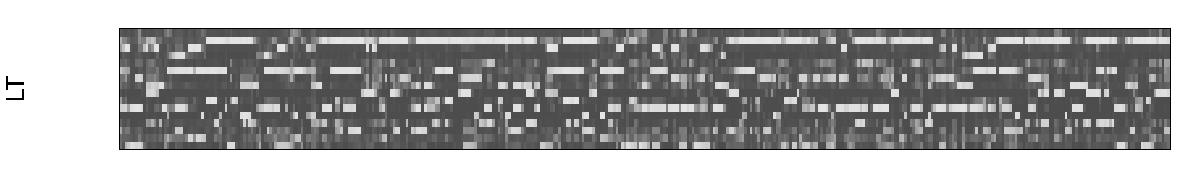
\includegraphics[width = \textwidth, height = 0.2\textwidth]{fig/cocktail/synth_s16_m12/hyper_gamma/h10.0_nocs_cp0/a5b0p01/LT_hdp_hmm_w0_agamma5_bgamma0p01/binary_state.pdf}}
  \centerline{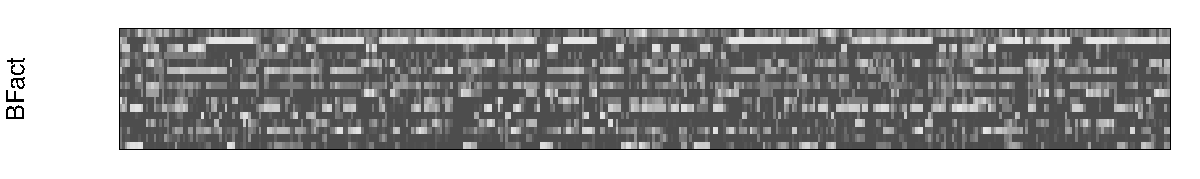
\includegraphics[width = \textwidth, height = 0.2\textwidth]{fig/cocktail/synth_s16_m12/hyper_gamma/h10.0_nocs_cp0/a5b0p01/BFact_hmm_w0_agamma5_bgamma0p01/binary_state.pdf}}
  \centerline{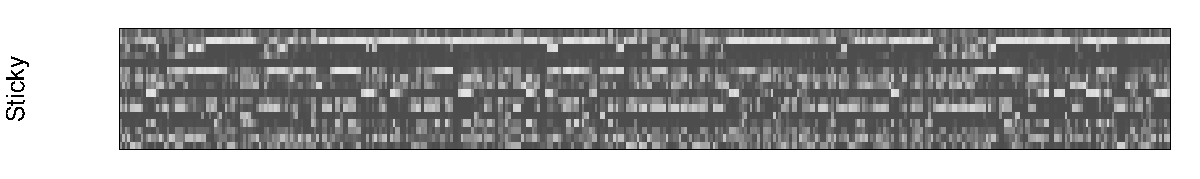
\includegraphics[width = \textwidth, height = 0.2\textwidth]{fig/cocktail/synth_s16_m12/hyper_gamma/h10.0_nocs_cp0/a5b0p01/Sticky_hdp_hmm_w0_agamma5_bgamma0p01/binary_state.pdf}}
  \centerline{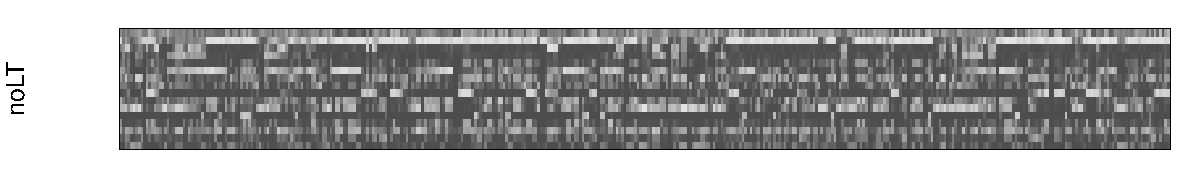
\includegraphics[width = \textwidth, height = 0.2\textwidth]{fig/cocktail/synth_s16_m12/hyper_gamma/h10.0_nocs_cp0/a5b0p01/noLT_hdp_hmm_w0_agamma5_bgamma0p01/binary_state.pdf}}
\caption{Binary speaker matrices for run 3: $\gamma \sim \Gamm{5}{0.01}$}
\end{center}
\end{figure}

\begin{figure}[tb]
  \centering
  \begin{minipage}{0.75\textwidth}
  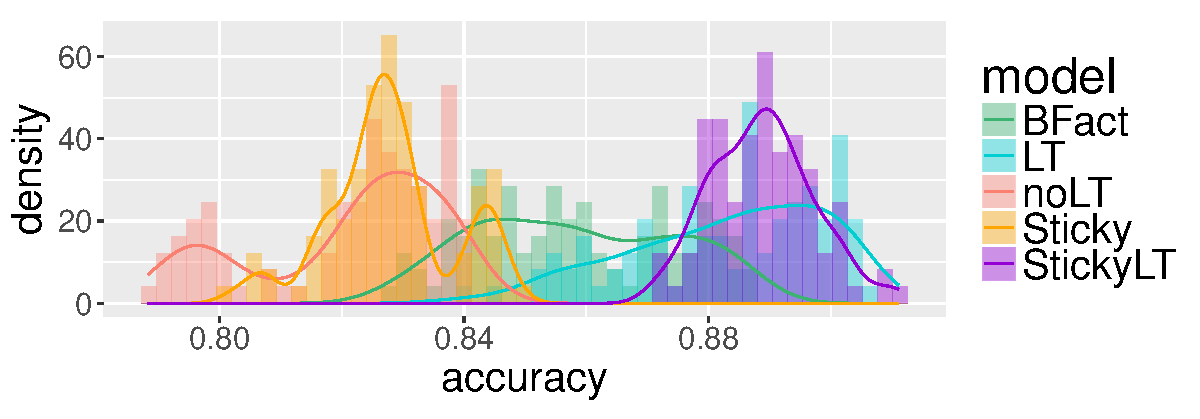
\includegraphics[width = \textwidth]{fig/cocktail/synth_s16_m12/hyper_gamma/h10.0_nocs_cp0/a5b5/accuracy_density.pdf}
\end{minipage}

\begin{minipage}{0.75\textwidth}
  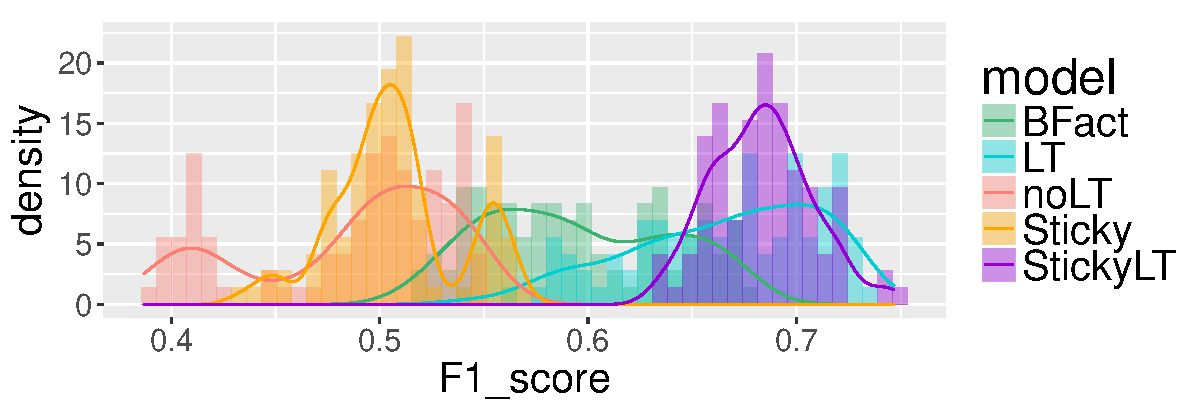
\includegraphics[width = \textwidth]{fig/cocktail/synth_s16_m12/hyper_gamma/h10.0_nocs_cp0/a5b5/F1_score_density.pdf}
\end{minipage}

\begin{minipage}{0.75\textwidth}
  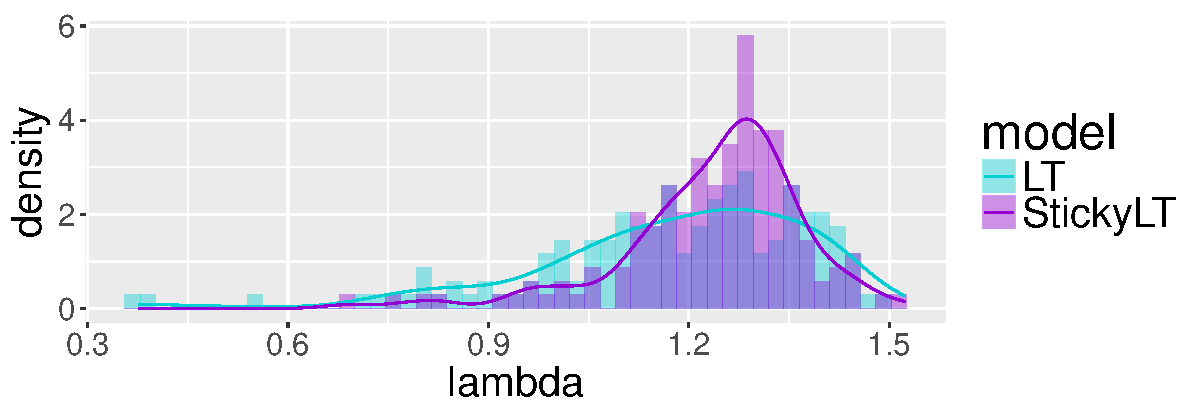
\includegraphics[width = \textwidth]{fig/cocktail/synth_s16_m12/hyper_gamma/h10.0_nocs_cp0/a5b5/lambda_density.pdf}
\end{minipage}

\begin{minipage}{0.75\textwidth}
  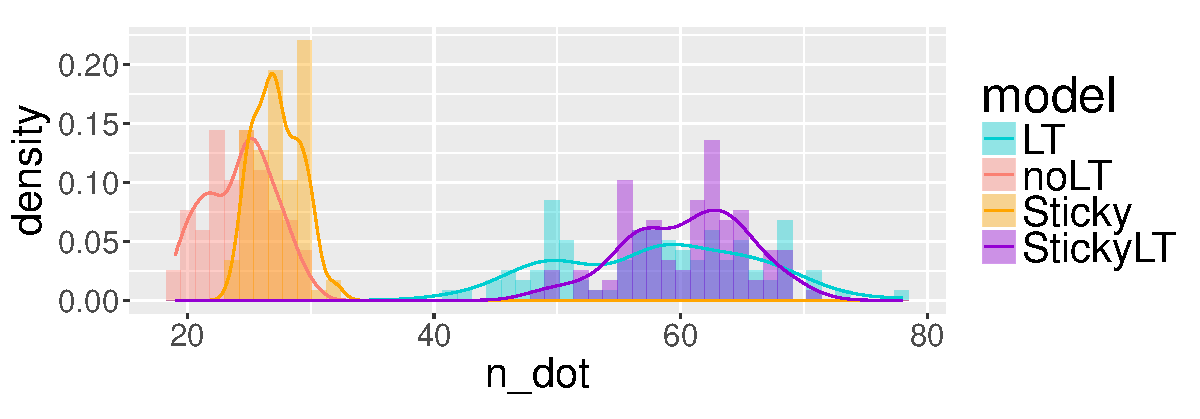
\includegraphics[width = \textwidth]{fig/cocktail/synth_s16_m12/hyper_gamma/h10.0_nocs_cp0/a5b5/n_dot_density.pdf}
\end{minipage}
\caption{Metrics for run 4: $\gamma \sim \Gamm{5}{5}$}
\end{figure}

\begin{figure}[tb]
% \vskip 0.1in
\begin{center}
  \centerline{\includegraphics[width = \textwidth, height = 0.2\textwidth]{fig/cocktail/synth_s16_m12/hyper_gamma/h10.0_nocs_cp0/a5b5/groundtruth.pdf}}
  \centerline{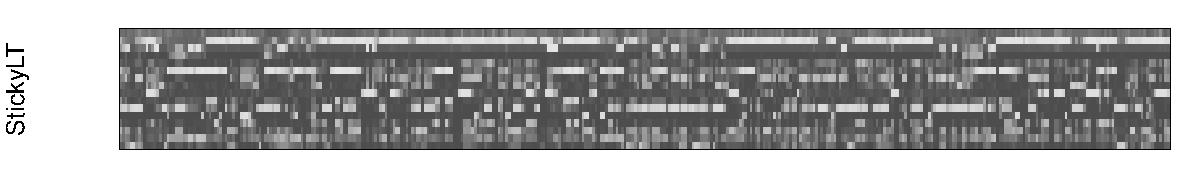
\includegraphics[width = \textwidth, height = 0.2\textwidth]{fig/cocktail/synth_s16_m12/hyper_gamma/h10.0_nocs_cp0/a5b5/StickyLT_hdp_hmm_w0_agamma5_bgamma5/binary_state.pdf}}
  \centerline{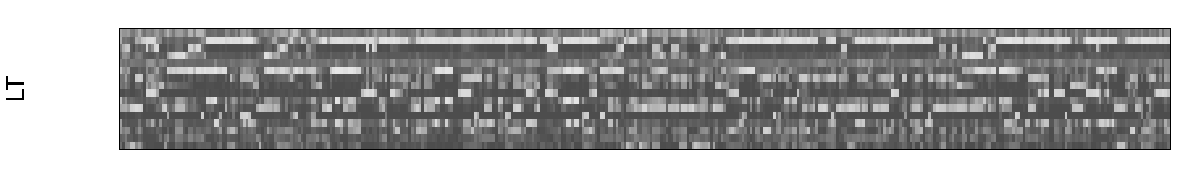
\includegraphics[width = \textwidth, height = 0.2\textwidth]{fig/cocktail/synth_s16_m12/hyper_gamma/h10.0_nocs_cp0/a5b5/LT_hdp_hmm_w0_agamma5_bgamma5/binary_state.pdf}}
  \centerline{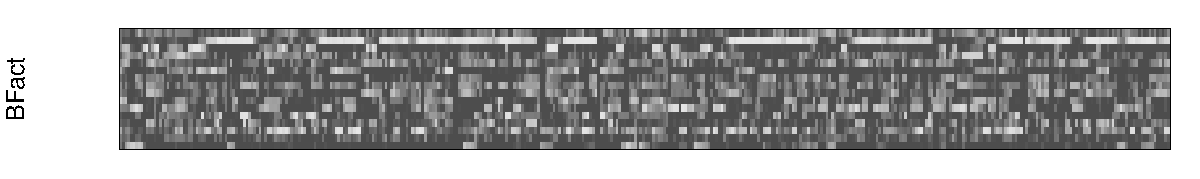
\includegraphics[width = \textwidth, height = 0.2\textwidth]{fig/cocktail/synth_s16_m12/hyper_gamma/h10.0_nocs_cp0/a5b5/BFact_hmm_w0_agamma5_bgamma5/binary_state.pdf}}
  \centerline{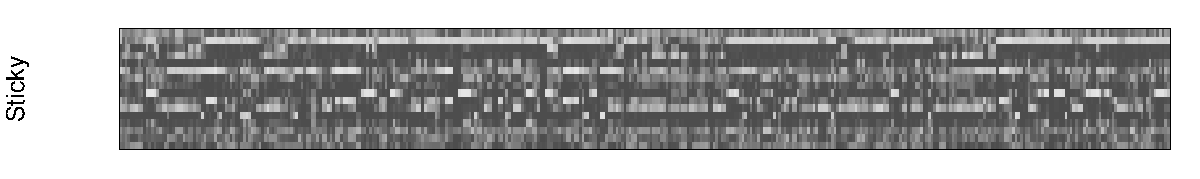
\includegraphics[width = \textwidth, height = 0.2\textwidth]{fig/cocktail/synth_s16_m12/hyper_gamma/h10.0_nocs_cp0/a5b5/Sticky_hdp_hmm_w0_agamma5_bgamma5/binary_state.pdf}}
  \centerline{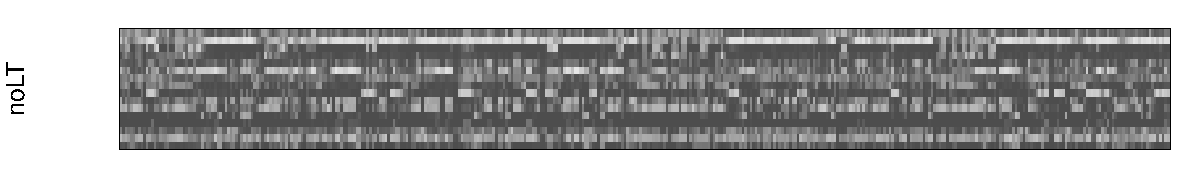
\includegraphics[width = \textwidth, height = 0.2\textwidth]{fig/cocktail/synth_s16_m12/hyper_gamma/h10.0_nocs_cp0/a5b5/noLT_hdp_hmm_w0_agamma5_bgamma5/binary_state.pdf}}
\caption{Binary speaker matrices for run 4: $\gamma \sim \Gamm{5}{5}$}
\end{center}
\end{figure}


\begin{figure}[tb]
  \centering
  \begin{minipage}{0.75\textwidth}
  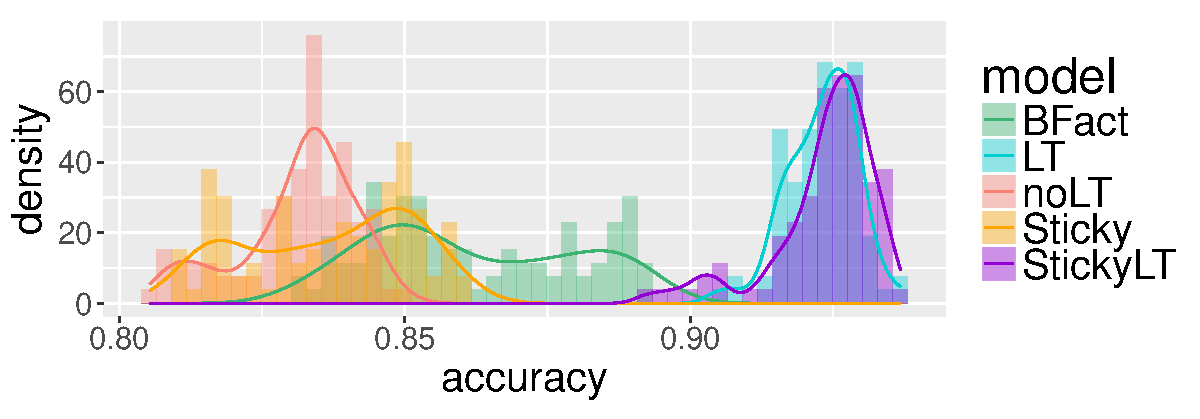
\includegraphics[width = \textwidth]{fig/cocktail/synth_s16_m12/hyper_alpha/h10.0_nocs_cp0/a0p01b0p01/accuracy_density.pdf}
\end{minipage}

\begin{minipage}{0.75\textwidth}
  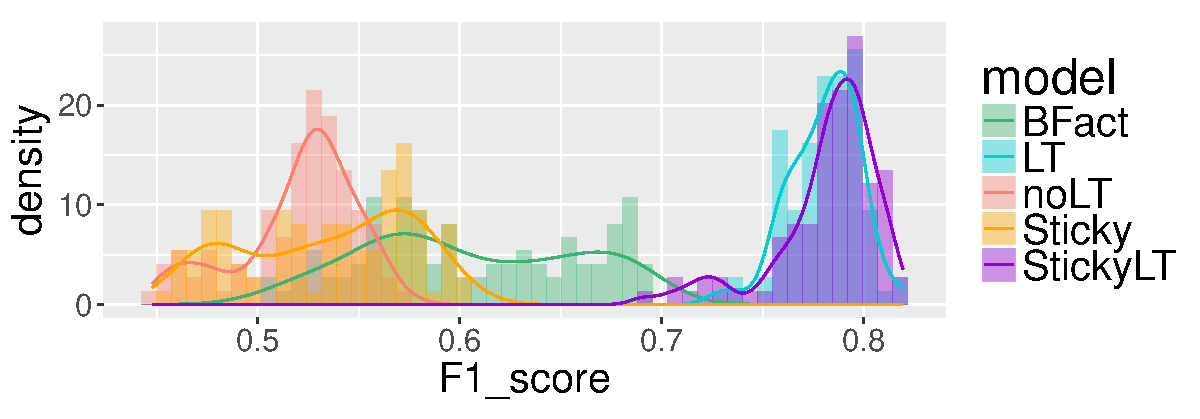
\includegraphics[width = \textwidth]{fig/cocktail/synth_s16_m12/hyper_alpha/h10.0_nocs_cp0/a0p01b0p01/F1_score_density.pdf}
\end{minipage}

\begin{minipage}{0.75\textwidth}
  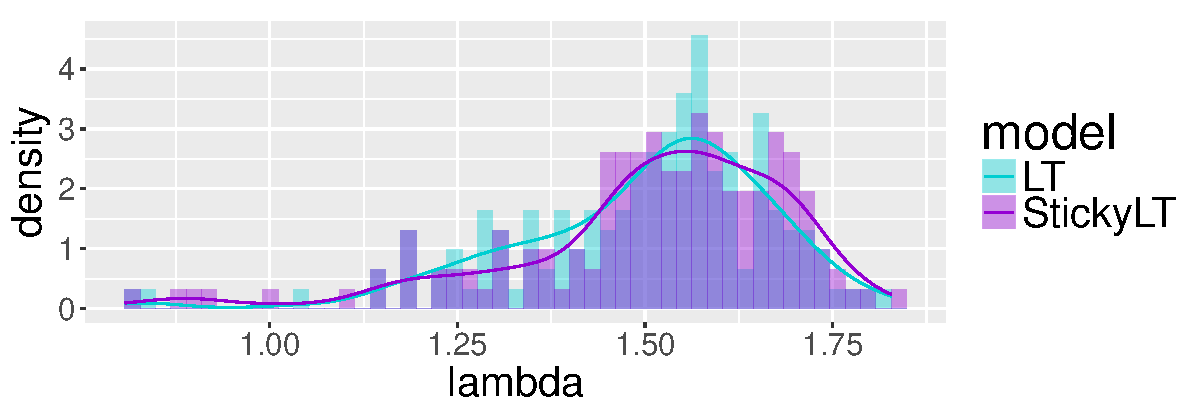
\includegraphics[width = \textwidth]{fig/cocktail/synth_s16_m12/hyper_alpha/h10.0_nocs_cp0/a0p01b0p01/lambda_density.pdf}
\end{minipage}

\begin{minipage}{0.75\textwidth}
  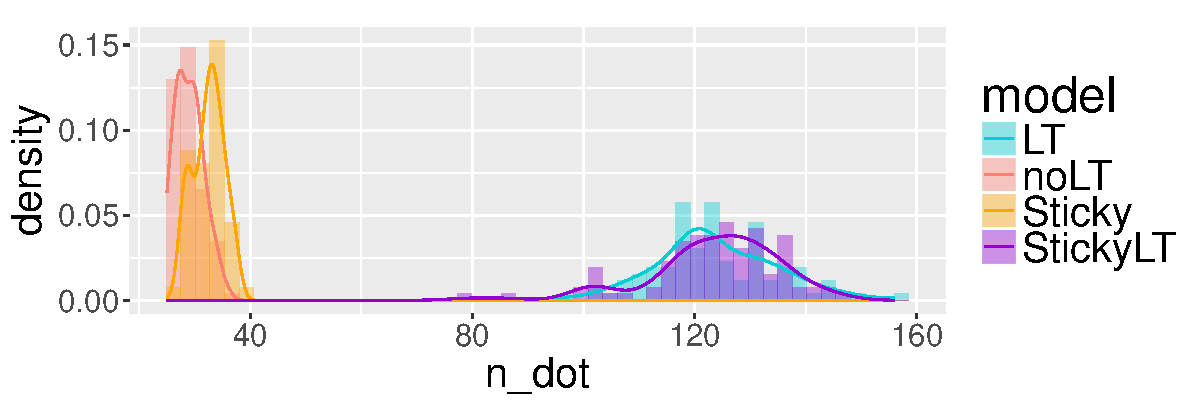
\includegraphics[width = \textwidth]{fig/cocktail/synth_s16_m12/hyper_alpha/h10.0_nocs_cp0/a0p01b0p01/n_dot_density.pdf}
\end{minipage}
\caption{Metrics for run 5: $\alpha \sim \Gamm{0.01}{0.01}$}
\end{figure}

\begin{figure}[tb]
% \vskip 0.1in
\begin{center}
  \centerline{\includegraphics[width = \textwidth, height = 0.2\textwidth]{fig/cocktail/synth_s16_m12/hyper_alpha/h10.0_nocs_cp0/a0p01b0p01/groundtruth.pdf}}
  \centerline{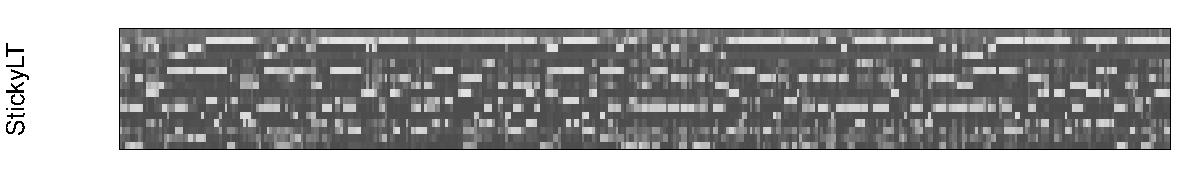
\includegraphics[width = \textwidth, height = 0.2\textwidth]{fig/cocktail/synth_s16_m12/hyper_alpha/h10.0_nocs_cp0/a0p01b0p01/StickyLT_hdp_hmm_w0_aalpha0p01_balpha0p01/binary_state.pdf}}
  \centerline{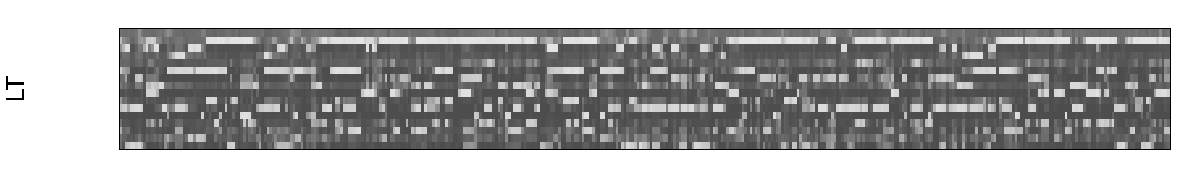
\includegraphics[width = \textwidth, height = 0.2\textwidth]{fig/cocktail/synth_s16_m12/hyper_alpha/h10.0_nocs_cp0/a0p01b0p01/LT_hdp_hmm_w0_aalpha0p01_balpha0p01/binary_state.pdf}}
  \centerline{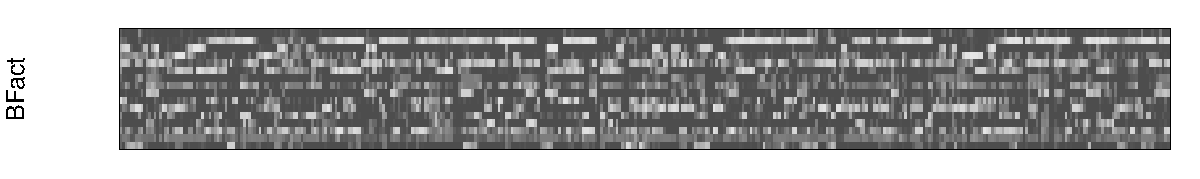
\includegraphics[width = \textwidth, height = 0.2\textwidth]{fig/cocktail/synth_s16_m12/hyper_alpha/h10.0_nocs_cp0/a0p01b0p01/BFact_hmm_w0_aalpha0p01_balpha0p01/binary_state.pdf}}
  \centerline{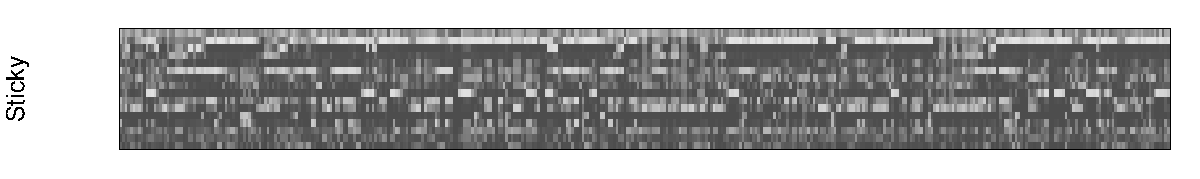
\includegraphics[width = \textwidth, height = 0.2\textwidth]{fig/cocktail/synth_s16_m12/hyper_alpha/h10.0_nocs_cp0/a0p01b0p01/Sticky_hdp_hmm_w0_aalpha0p01_balpha0p01/binary_state.pdf}}
  \centerline{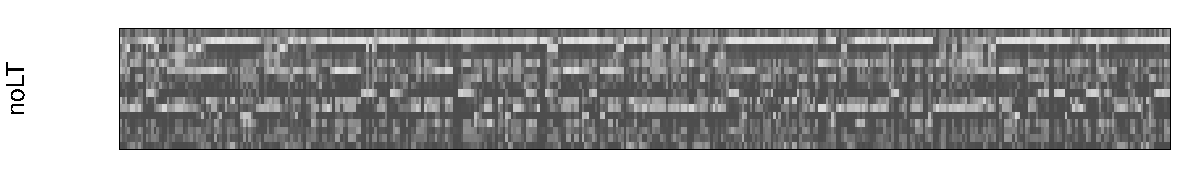
\includegraphics[width = \textwidth, height = 0.2\textwidth]{fig/cocktail/synth_s16_m12/hyper_alpha/h10.0_nocs_cp0/a0p01b0p01/noLT_hdp_hmm_w0_aalpha0p01_balpha0p01/binary_state.pdf}}
\caption{Binary speaker matrices for run 5: $\alpha \sim \Gamm{0.01}{0.01}$}
\end{center}
\end{figure}


\begin{figure}[tb]
  \centering
  \begin{minipage}{0.75\textwidth}
  \includegraphics[width = \textwidth]{fig/cocktail/synth_s16_m12/hyper_alpha/h10.0_nocs_cp0/a0p01b5/accuracy_density.pdf}
\end{minipage}

\begin{minipage}{0.75\textwidth}
  \includegraphics[width = \textwidth]{fig/cocktail/synth_s16_m12/hyper_alpha/h10.0_nocs_cp0/a0p01b5/F1_score_density.pdf}
\end{minipage}

\begin{minipage}{0.75\textwidth}
  \includegraphics[width = \textwidth]{fig/cocktail/synth_s16_m12/hyper_alpha/h10.0_nocs_cp0/a0p01b5/lambda_density.pdf}
\end{minipage}

\begin{minipage}{0.75\textwidth}
  \includegraphics[width = \textwidth]{fig/cocktail/synth_s16_m12/hyper_alpha/h10.0_nocs_cp0/a0p01b5/n_dot_density.pdf}
\end{minipage}
\caption{Metrics for run 6: $\alpha \sim \Gamm{0.01}{5}$}
\end{figure}

\begin{figure}[tb]
% \vskip 0.1in
\begin{center}
  \centerline{\includegraphics[width = \textwidth, height = 0.2\textwidth]{fig/cocktail/synth_s16_m12/hyper_alpha/h10.0_nocs_cp0/a0p01b5/groundtruth.pdf}}
  \centerline{\includegraphics[width = \textwidth, height = 0.2\textwidth]{fig/cocktail/synth_s16_m12/hyper_alpha/h10.0_nocs_cp0/a0p01b5/StickyLT_hdp_hmm_w0_aalpha0p01_balpha5/binary_state.pdf}}
  \centerline{\includegraphics[width = \textwidth, height = 0.2\textwidth]{fig/cocktail/synth_s16_m12/hyper_alpha/h10.0_nocs_cp0/a0p01b5/LT_hdp_hmm_w0_aalpha0p01_balpha5/binary_state.pdf}}
  \centerline{\includegraphics[width = \textwidth, height = 0.2\textwidth]{fig/cocktail/synth_s16_m12/hyper_alpha/h10.0_nocs_cp0/a0p01b5/BFact_hmm_w0_aalpha0p01_balpha5/binary_state.pdf}}
  \centerline{\includegraphics[width = \textwidth, height = 0.2\textwidth]{fig/cocktail/synth_s16_m12/hyper_alpha/h10.0_nocs_cp0/a0p01b5/Sticky_hdp_hmm_w0_aalpha0p01_balpha5/binary_state.pdf}}
  \centerline{\includegraphics[width = \textwidth, height = 0.2\textwidth]{fig/cocktail/synth_s16_m12/hyper_alpha/h10.0_nocs_cp0/a0p01b5/noLT_hdp_hmm_w0_aalpha0p01_balpha5/binary_state.pdf}}
\caption{Binary speaker matrices for run 6: $\alpha \sim \Gamm{0.01}{5}$}
\end{center}
\end{figure}

\begin{figure}[tb]
  \centering
  \begin{minipage}{0.75\textwidth}
  \includegraphics[width = \textwidth]{fig/cocktail/synth_s16_m12/hyper_alpha/h10.0_nocs_cp0/a5b0p01/accuracy_density.pdf}
\end{minipage}

\begin{minipage}{0.75\textwidth}
  \includegraphics[width = \textwidth]{fig/cocktail/synth_s16_m12/hyper_alpha/h10.0_nocs_cp0/a5b0p01/F1_score_density.pdf}
\end{minipage}

\begin{minipage}{0.75\textwidth}
  \includegraphics[width = \textwidth]{fig/cocktail/synth_s16_m12/hyper_alpha/h10.0_nocs_cp0/a5b0p01/lambda_density.pdf}
\end{minipage}

\begin{minipage}{0.75\textwidth}
  \includegraphics[width = \textwidth]{fig/cocktail/synth_s16_m12/hyper_alpha/h10.0_nocs_cp0/a5b0p01/n_dot_density.pdf}
\end{minipage}
\caption{Metrics for run 7: $\alpha \sim \Gamm{5}{0.01}$}
\end{figure}

\begin{figure}[tb]
% \vskip 0.1in
\begin{center}
  \centerline{\includegraphics[width = \textwidth, height = 0.2\textwidth]{fig/cocktail/synth_s16_m12/hyper_alpha/h10.0_nocs_cp0/a5b0p01/groundtruth.pdf}}
  \centerline{\includegraphics[width = \textwidth, height = 0.2\textwidth]{fig/cocktail/synth_s16_m12/hyper_alpha/h10.0_nocs_cp0/a5b0p01/StickyLT_hdp_hmm_w0_aalpha5_balpha0p01/binary_state.pdf}}
  \centerline{\includegraphics[width = \textwidth, height = 0.2\textwidth]{fig/cocktail/synth_s16_m12/hyper_alpha/h10.0_nocs_cp0/a5b0p01/LT_hdp_hmm_w0_aalpha5_balpha0p01/binary_state.pdf}}
  \centerline{\includegraphics[width = \textwidth, height = 0.2\textwidth]{fig/cocktail/synth_s16_m12/hyper_alpha/h10.0_nocs_cp0/a5b0p01/BFact_hmm_w0_aalpha5_balpha0p01/binary_state.pdf}}
  \centerline{\includegraphics[width = \textwidth, height = 0.2\textwidth]{fig/cocktail/synth_s16_m12/hyper_alpha/h10.0_nocs_cp0/a5b0p01/Sticky_hdp_hmm_w0_aalpha5_balpha0p01/binary_state.pdf}}
  \centerline{\includegraphics[width = \textwidth, height = 0.2\textwidth]{fig/cocktail/synth_s16_m12/hyper_alpha/h10.0_nocs_cp0/a5b0p01/noLT_hdp_hmm_w0_aalpha5_balpha0p01/binary_state.pdf}}
\caption{Binary speaker matrices for run 7: $\alpha \sim \Gamm{5}{0.01}$}
\end{center}
\end{figure}

\begin{figure}[tb]
  \centering
  \begin{minipage}{0.75\textwidth}
  \includegraphics[width = \textwidth]{fig/cocktail/synth_s16_m12/hyper_alpha/h10.0_nocs_cp0/a5b5/accuracy_density.pdf}
\end{minipage}

\begin{minipage}{0.75\textwidth}
  \includegraphics[width = \textwidth]{fig/cocktail/synth_s16_m12/hyper_alpha/h10.0_nocs_cp0/a5b5/F1_score_density.pdf}
\end{minipage}

\begin{minipage}{0.75\textwidth}
  \includegraphics[width = \textwidth]{fig/cocktail/synth_s16_m12/hyper_alpha/h10.0_nocs_cp0/a5b5/lambda_density.pdf}
\end{minipage}

\begin{minipage}{0.75\textwidth}
  \includegraphics[width = \textwidth]{fig/cocktail/synth_s16_m12/hyper_alpha/h10.0_nocs_cp0/a5b5/n_dot_density.pdf}
\end{minipage}
\caption{Metrics for run 8: $\alpha \sim \Gamm{5}{5}$}
\end{figure}

\begin{figure}[tb]
% \vskip 0.1in
\begin{center}
  \centerline{\includegraphics[width = \textwidth, height = 0.2\textwidth]{fig/cocktail/synth_s16_m12/hyper_alpha/h10.0_nocs_cp0/a5b5/groundtruth.pdf}}
  \centerline{\includegraphics[width = \textwidth, height = 0.2\textwidth]{fig/cocktail/synth_s16_m12/hyper_alpha/h10.0_nocs_cp0/a5b5/StickyLT_hdp_hmm_w0_aalpha5_balpha5/binary_state.pdf}}
  \centerline{\includegraphics[width = \textwidth, height = 0.2\textwidth]{fig/cocktail/synth_s16_m12/hyper_alpha/h10.0_nocs_cp0/a5b5/LT_hdp_hmm_w0_aalpha5_balpha5/binary_state.pdf}}
  \centerline{\includegraphics[width = \textwidth, height = 0.2\textwidth]{fig/cocktail/synth_s16_m12/hyper_alpha/h10.0_nocs_cp0/a5b5/BFact_hmm_w0_aalpha5_balpha5/binary_state.pdf}}
  \centerline{\includegraphics[width = \textwidth, height = 0.2\textwidth]{fig/cocktail/synth_s16_m12/hyper_alpha/h10.0_nocs_cp0/a5b5/Sticky_hdp_hmm_w0_aalpha5_balpha5/binary_state.pdf}}
  \centerline{\includegraphics[width = \textwidth, height = 0.2\textwidth]{fig/cocktail/synth_s16_m12/hyper_alpha/h10.0_nocs_cp0/a5b5/noLT_hdp_hmm_w0_aalpha5_balpha5/binary_state.pdf}}
\caption{Binary speaker matrices for run 8: $\alpha \sim \Gamm{5}{5}$}
\end{center}
\end{figure}


\begin{figure}[tb]
  \centering
  \begin{minipage}{0.75\textwidth}
  \includegraphics[width = \textwidth]{fig/cocktail/synth_s16_m12/hyper_h/h10.0_nocs_cp0/a0p01b0p01/accuracy_density.pdf}
\end{minipage}

\begin{minipage}{0.75\textwidth}
  \includegraphics[width = \textwidth]{fig/cocktail/synth_s16_m12/hyper_h/h10.0_nocs_cp0/a0p01b0p01/F1_score_density.pdf}
\end{minipage}

\begin{minipage}{0.75\textwidth}
  \includegraphics[width = \textwidth]{fig/cocktail/synth_s16_m12/hyper_h/h10.0_nocs_cp0/a0p01b0p01/lambda_density.pdf}
\end{minipage}

\begin{minipage}{0.75\textwidth}
  \includegraphics[width = \textwidth]{fig/cocktail/synth_s16_m12/hyper_h/h10.0_nocs_cp0/a0p01b0p01/n_dot_density.pdf}
\end{minipage}
\caption{Metrics for run 9: $h \sim \Gamm{0.01}{0.01}$}
\end{figure}

\begin{figure}[tb]
% \vskip 0.1in
\begin{center}
  \centerline{\includegraphics[width = \textwidth, height = 0.2\textwidth]{fig/cocktail/synth_s16_m12/hyper_h/h10.0_nocs_cp0/a0p01b0p01/groundtruth.pdf}}
  \centerline{\includegraphics[width = \textwidth, height = 0.2\textwidth]{fig/cocktail/synth_s16_m12/hyper_h/h10.0_nocs_cp0/a0p01b0p01/StickyLT_hdp_hmm_w0_ah0p01_bh0p01/binary_state.pdf}}
  \centerline{\includegraphics[width = \textwidth, height = 0.2\textwidth]{fig/cocktail/synth_s16_m12/hyper_h/h10.0_nocs_cp0/a0p01b0p01/LT_hdp_hmm_w0_ah0p01_bh0p01/binary_state.pdf}}
  \centerline{\includegraphics[width = \textwidth, height = 0.2\textwidth]{fig/cocktail/synth_s16_m12/hyper_h/h10.0_nocs_cp0/a0p01b0p01/BFact_hmm_w0_ah0p01_bh0p01/binary_state.pdf}}
  \centerline{\includegraphics[width = \textwidth, height = 0.2\textwidth]{fig/cocktail/synth_s16_m12/hyper_h/h10.0_nocs_cp0/a0p01b0p01/Sticky_hdp_hmm_w0_ah0p01_bh0p01/binary_state.pdf}}
  \centerline{\includegraphics[width = \textwidth, height = 0.2\textwidth]{fig/cocktail/synth_s16_m12/hyper_h/h10.0_nocs_cp0/a0p01b0p01/noLT_hdp_hmm_w0_ah0p01_bh0p01/binary_state.pdf}}
\caption{Binary speaker matrices for run 9: $h \sim \Gamm{0.01}{0.01}$}
\end{center}
\end{figure}


\begin{figure}[tb]
  \centering
  \begin{minipage}{0.75\textwidth}
  \includegraphics[width = \textwidth]{fig/cocktail/synth_s16_m12/hyper_h/h10.0_nocs_cp0/a0p01b5/accuracy_density.pdf}
\end{minipage}

\begin{minipage}{0.75\textwidth}
  \includegraphics[width = \textwidth]{fig/cocktail/synth_s16_m12/hyper_h/h10.0_nocs_cp0/a0p01b5/F1_score_density.pdf}
\end{minipage}

\begin{minipage}{0.75\textwidth}
  \includegraphics[width = \textwidth]{fig/cocktail/synth_s16_m12/hyper_h/h10.0_nocs_cp0/a0p01b5/lambda_density.pdf}
\end{minipage}

\begin{minipage}{0.75\textwidth}
  \includegraphics[width = \textwidth]{fig/cocktail/synth_s16_m12/hyper_h/h10.0_nocs_cp0/a0p01b5/n_dot_density.pdf}
\end{minipage}
\caption{Metrics for run 10: $h \sim \Gamm{0.01}{5}$}
\end{figure}

\begin{figure}[tb]
% \vskip 0.1in
\begin{center}
  \centerline{\includegraphics[width = \textwidth, height = 0.2\textwidth]{fig/cocktail/synth_s16_m12/hyper_h/h10.0_nocs_cp0/a0p01b5/groundtruth.pdf}}
  \centerline{\includegraphics[width = \textwidth, height = 0.2\textwidth]{fig/cocktail/synth_s16_m12/hyper_h/h10.0_nocs_cp0/a0p01b5/StickyLT_hdp_hmm_w0_ah0p01_bh5/binary_state.pdf}}
  \centerline{\includegraphics[width = \textwidth, height = 0.2\textwidth]{fig/cocktail/synth_s16_m12/hyper_h/h10.0_nocs_cp0/a0p01b5/LT_hdp_hmm_w0_ah0p01_bh5/binary_state.pdf}}
  \centerline{\includegraphics[width = \textwidth, height = 0.2\textwidth]{fig/cocktail/synth_s16_m12/hyper_h/h10.0_nocs_cp0/a0p01b5/BFact_hmm_w0_ah0p01_bh5/binary_state.pdf}}
  \centerline{\includegraphics[width = \textwidth, height = 0.2\textwidth]{fig/cocktail/synth_s16_m12/hyper_h/h10.0_nocs_cp0/a0p01b5/Sticky_hdp_hmm_w0_ah0p01_bh5/binary_state.pdf}}
  \centerline{\includegraphics[width = \textwidth, height = 0.2\textwidth]{fig/cocktail/synth_s16_m12/hyper_h/h10.0_nocs_cp0/a0p01b5/noLT_hdp_hmm_w0_ah0p01_bh5/binary_state.pdf}}
\caption{Binary speaker matrices for run 10: $h \sim \Gamm{0.01}{5}$}
\end{center}
\end{figure}

\begin{figure}[tb]
  \centering
  \begin{minipage}{0.75\textwidth}
  \includegraphics[width = \textwidth]{fig/cocktail/synth_s16_m12/hyper_h/h10.0_nocs_cp0/a5b0p01/accuracy_density.pdf}
\end{minipage}

\begin{minipage}{0.75\textwidth}
  \includegraphics[width = \textwidth]{fig/cocktail/synth_s16_m12/hyper_h/h10.0_nocs_cp0/a5b0p01/F1_score_density.pdf}
\end{minipage}

\begin{minipage}{0.75\textwidth}
  \includegraphics[width = \textwidth]{fig/cocktail/synth_s16_m12/hyper_h/h10.0_nocs_cp0/a5b0p01/lambda_density.pdf}
\end{minipage}

\begin{minipage}{0.75\textwidth}
  \includegraphics[width = \textwidth]{fig/cocktail/synth_s16_m12/hyper_h/h10.0_nocs_cp0/a5b0p01/n_dot_density.pdf}
\end{minipage}
\caption{Metrics for run 11: $h \sim \Gamm{5}{0.01}$}
\end{figure}

\begin{figure}[tb]
% \vskip 0.1in
\begin{center}
  \centerline{\includegraphics[width = \textwidth, height = 0.2\textwidth]{fig/cocktail/synth_s16_m12/hyper_h/h10.0_nocs_cp0/a5b0p01/groundtruth.pdf}}
  \centerline{\includegraphics[width = \textwidth, height = 0.2\textwidth]{fig/cocktail/synth_s16_m12/hyper_h/h10.0_nocs_cp0/a5b0p01/StickyLT_hdp_hmm_w0_ah5_bh0p01/binary_state.pdf}}
  \centerline{\includegraphics[width = \textwidth, height = 0.2\textwidth]{fig/cocktail/synth_s16_m12/hyper_h/h10.0_nocs_cp0/a5b0p01/LT_hdp_hmm_w0_ah5_bh0p01/binary_state.pdf}}
  \centerline{\includegraphics[width = \textwidth, height = 0.2\textwidth]{fig/cocktail/synth_s16_m12/hyper_h/h10.0_nocs_cp0/a5b0p01/BFact_hmm_w0_ah5_bh0p01/binary_state.pdf}}
  \centerline{\includegraphics[width = \textwidth, height = 0.2\textwidth]{fig/cocktail/synth_s16_m12/hyper_h/h10.0_nocs_cp0/a5b0p01/Sticky_hdp_hmm_w0_ah5_bh0p01/binary_state.pdf}}
  \centerline{\includegraphics[width = \textwidth, height = 0.2\textwidth]{fig/cocktail/synth_s16_m12/hyper_h/h10.0_nocs_cp0/a5b0p01/noLT_hdp_hmm_w0_ah5_bh0p01/binary_state.pdf}}
\caption{Binary speaker matrices for run 11: $h \sim \Gamm{5}{0.01}$}
\end{center}
\end{figure}

\begin{figure}[tb]
  \centering
  \begin{minipage}{0.75\textwidth}
  \includegraphics[width = \textwidth]{fig/cocktail/synth_s16_m12/hyper_h/h10.0_nocs_cp0/a5b5/accuracy_density.pdf}
\end{minipage}

\begin{minipage}{0.75\textwidth}
  \includegraphics[width = \textwidth]{fig/cocktail/synth_s16_m12/hyper_h/h10.0_nocs_cp0/a5b5/F1_score_density.pdf}
\end{minipage}

\begin{minipage}{0.75\textwidth}
  \includegraphics[width = \textwidth]{fig/cocktail/synth_s16_m12/hyper_h/h10.0_nocs_cp0/a5b5/lambda_density.pdf}
\end{minipage}

\begin{minipage}{0.75\textwidth}
  \includegraphics[width = \textwidth]{fig/cocktail/synth_s16_m12/hyper_h/h10.0_nocs_cp0/a5b5/n_dot_density.pdf}
\end{minipage}
\caption{Metrics for run 12: $h \sim \Gamm{5}{5}$}
\end{figure}

\begin{figure}[tb]
% \vskip 0.1in
\begin{center}
  \centerline{\includegraphics[width = \textwidth, height = 0.2\textwidth]{fig/cocktail/synth_s16_m12/hyper_h/h10.0_nocs_cp0/a5b5/groundtruth.pdf}}
  \centerline{\includegraphics[width = \textwidth, height = 0.2\textwidth]{fig/cocktail/synth_s16_m12/hyper_h/h10.0_nocs_cp0/a5b5/StickyLT_hdp_hmm_w0_ah5_bh5/binary_state.pdf}}
  \centerline{\includegraphics[width = \textwidth, height = 0.2\textwidth]{fig/cocktail/synth_s16_m12/hyper_h/h10.0_nocs_cp0/a5b5/LT_hdp_hmm_w0_ah5_bh5/binary_state.pdf}}
  \centerline{\includegraphics[width = \textwidth, height = 0.2\textwidth]{fig/cocktail/synth_s16_m12/hyper_h/h10.0_nocs_cp0/a5b5/BFact_hmm_w0_ah5_bh5/binary_state.pdf}}
  \centerline{\includegraphics[width = \textwidth, height = 0.2\textwidth]{fig/cocktail/synth_s16_m12/hyper_h/h10.0_nocs_cp0/a5b5/Sticky_hdp_hmm_w0_ah5_bh5/binary_state.pdf}}
  \centerline{\includegraphics[width = \textwidth, height = 0.2\textwidth]{fig/cocktail/synth_s16_m12/hyper_h/h10.0_nocs_cp0/a5b5/noLT_hdp_hmm_w0_ah5_bh5/binary_state.pdf}}
\caption{Binary speaker matrices for run 12: $h \sim \Gamm{5}{5}$}
\end{center}
\end{figure}

\section{Bach Chorale Data}

The models used in the music experiments in Chapter \ref{chapter:music}
employ separate emission and similarity spaces, and hence, conditioned
on the state sequence, the observations do not inform the locations,
$\ell_j$.  As a result there is no extrinsic information about the
scale of the similarity kernel, since performing a rescaling of the
locations $\ell_j$ together with an inverse scaling of the kernel
parameter $\lambda$ results in an equivalent likelihood.  Therefore,
rather than letting $\lambda$ be inferred as it is in the cocktail
party experiments, its value was fixed, whereas the locations are
given a multivariate $\Norm{0}{\mathbf{I}}$ prior (in all experiments
reported here the dimension of the similarity space is $2$)
and are sampled using Hamiltonian Monte Carlo.

Although sampling state locations in principle allows similarities to be learned,
the choice of scale parameter $\lambda$ relative to the prior on state
locations is consequential in practice.  In
Figs. \ref{fig:bach-hyperparameter-lambda0p01}-\ref{fig:bach-hyperparameter-lambda5p0},
training and test set log likelihoods are shown on the Bach chorale data for four models ---
HDP-HMM, Sticky HDP-HMM, HDP-HMM-LT, and Sticky HDP-HMM-LT --- with
$\lambda$ values of 0.01, 1.0 and 5.0, respectively.  In
Fig. \ref{fig:bach-hyperparameter-all-lambdas}, the effect of
$\lambda$ on the log likelihood is shown for a spectrum of models
ranging from the original HDP-HMM ($\lambda = 0$) to an HDP-HMM-LT
with $\lambda = 10$.

The pattern reported in Chapter \ref{chapter:music} can be seen
clearly in these results: with very small $\lambda$ (0.01), the LT
models are nearly identical to the non-LT models.  As $\lambda$
increases up to 5, the gap increases, with the LT models achieving
lower training log likelihoods and higher test log likelihoods,
reflecting the tendency of the non-LT models' less restrictive prior on transition
matrices to overfit by employing as many states as possible.  When
$\lambda$ gets as large as 10, however, performance degrades, with
both training and test log likelihoods decreasing.  This likely
reflects a too-strong bias toward self-transitions, resulting in the
use of too few states and underfitting the data.

\begin{figure}[tb]
% \vskip 0.1in
\begin{center}
  \centerline{\includegraphics[width = 0.75\columnwidth]{fig/music/bach/lambda0p01/train_log_likelihood_density.pdf}}
  \centerline{\includegraphics[width = 0.75\columnwidth]{fig/music/bach/lambda0p01/test_log_likelihood_density.pdf}}
  \centerline{\includegraphics[width = 0.75\columnwidth]{fig/music/bach/lambda0p01/n_dot_density.pdf}}
  % \centerline{\includegraphics[width = \columnwidth]{fig/bach/alpha.pdf}}
\caption{Top and Middle: Training set and test set log marginal likelihoods for Bach
  chorale data on the four HDP-based models: HDP-HMM-LT, HDP-HMM,
  Sticky HMM, and Sticky HDP-HMM-LT, where the two LT models set
  $\lambda = 0.01$.  Bottom: Number of latent states
  occupied in the training set by each model. \label{fig:bach-hyperparameter-lambda0p01}
}
\end{center}
% \vskip 0.1in
\end{figure}

\begin{figure}[tb]
% \vskip 0.1in
\begin{center}
  \centerline{\includegraphics[width = 0.75\columnwidth]{fig/music/bach/lambda1/train_log_likelihood_density.pdf}}
  \centerline{\includegraphics[width = 0.75\columnwidth]{fig/music/bach/lambda1/test_log_likelihood_density.pdf}}
  \centerline{\includegraphics[width = 0.75\columnwidth]{fig/music/bach/lambda1/n_dot_density.pdf}}
  % \centerline{\includegraphics[width = \columnwidth]{fig/bach/alpha.pdf}}
\caption{Top and Middle: Training set and test set log marginal likelihoods for Bach
  chorale data on the four HDP-based models: HDP-HMM-LT, HDP-HMM,
  Sticky HMM, and Sticky HDP-HMM-LT, where the two LT models set
  $\lambda = 1.0$.  Bottom: Number of latent states
  occupied in the training set by each model. \label{fig:bach-hyperparameter-lambda1p0}
}
\end{center}
% \vskip 0.1in
\end{figure}

\begin{figure}[tb]
% \vskip 0.1in
\begin{center}
  \centerline{\includegraphics[width = 0.75\columnwidth]{fig/music/bach/lambda5/train_log_likelihood_density.pdf}}
  \centerline{\includegraphics[width = 0.75\columnwidth]{fig/music/bach/lambda5/test_log_likelihood_density.pdf}}
  \centerline{\includegraphics[width = 0.75\columnwidth]{fig/music/bach/lambda5/n_dot_density.pdf}}
  % \centerline{\includegraphics[width = \columnwidth]{fig/bach/alpha.pdf}}
\caption{Top and Middle: Training set and test set log marginal likelihoods for Bach
  chorale data on the four HDP-based models: HDP-HMM-LT, HDP-HMM,
  Sticky HMM, and Sticky HDP-HMM-LT, where the two LT models set
  $\lambda = 1.0$.  Bottom: Number of latent states
  occupied in the training set by each model. \label{fig:bach-hyperparameter-lambda5p0}
}
\end{center}
% \vskip 0.1in
\end{figure}

\begin{figure}[tb]
% \vskip 0.1in
\begin{center}
  \centerline{\includegraphics[width = 0.75\columnwidth]{fig/music/bach/varying_lambda_eps0005/train_log_likelihood_density.pdf}}
  \centerline{\includegraphics[width = 0.75\columnwidth]{fig/music/bach/varying_lambda_eps0005/test_log_likelihood_density.pdf}}
  \centerline{\includegraphics[width = 0.75\columnwidth]{fig/music/bach/varying_lambda_eps0005/n_dot_density.pdf}}
  % \centerline{\includegraphics[width = \columnwidth]{fig/bach/alpha.pdf}}
\caption{Top and Middle: Training set and test set log marginal likelihoods for Bach
  chorale data on the four HDP-based models: HDP-HMM-LT, HDP-HMM,
  Sticky HMM, and Sticky HDP-HMM-LT, where the two LT models set
  $\lambda = 1.0$.  Bottom: Number of latent states
  occupied in the training set by each model. \label{fig:bach-hyperparameter-all-lambdas}
}
\end{center}
% \vskip 0.1in
\end{figure}
